\section{Probe Underperformance on GPT-OSS 20B}
\label{sec:ch8-gpt-oss}

Among the eight models of Section~\ref{sec:ch7-results}, GPT-OSS 20B is the only one whose chain-of-thought output cannot be disabled (Section~\ref{subsec:ch7-reasoning-traces}). In its runs, a reasoning output is generated after the prompt and before the tool call that states the routing decision. GPT-OSS 20B is also the only model where the probe is less accurate than the coordinator. This section analyzes its two runs in detail, to determine whether the hidden state at the last prompt token may be insufficient to predict the choice of the sub-agent when the reasoning output cannot be disabled.

\begin{table}[htbp]
    \centering
    \begin{tabular}{@{}lcccc@{}}
        \toprule
        \textbf{Dataset} & \textbf{\begin{tabular}[b]{@{}c@{}}probe\\AUC macro\end{tabular}} & \textbf{\begin{tabular}[b]{@{}c@{}}probe AUC macro,\\other seven models\end{tabular}} & \textbf{\begin{tabular}[b]{@{}c@{}}coordinator\\accuracy\end{tabular}} & \textbf{\begin{tabular}[b]{@{}c@{}}probe\\accuracy\end{tabular}} \\
        \midrule
        Single-turn & 0.915 & 0.974--0.989 & \textbf{0.818} & 0.689 \\
        Multi-turn  & 0.788 & 0.928--0.979 & \textbf{0.719} & 0.505 \\
        \bottomrule
    \end{tabular}
    \caption[\texttt{gpt-oss-20b} probe AUC macro and coordinator accuracy]{\texttt{gpt-oss-20b}: AUC macro of the probe at its optimal layer, range of the same metric across the other seven models, accuracy of the coordinator and accuracy of the probe, from Section~\ref{sec:ch7-results}.}
    \label{tab:ch8-gpt-oss-exception}
\end{table}

Table~\ref{tab:ch8-gpt-oss-exception} shows that the accuracy of the probe is lower than the accuracy of the coordinator by 0.129 on the single-turn dataset and by 0.214 on the multi-turn dataset. On both datasets, the AUC macro of the probe is also below the range of the other seven models. The sub-agents are therefore less separable in the hidden states of GPT-OSS 20B than in those of any other model analyzed in this work.

\subsection{Probing at the Last Reasoning Token}
\label{subsec:ch8-gpt-oss-reasoning}

The probe reads the hidden state at the last prompt token, before the reasoning output is generated. For the other seven models the tool call follows the prompt directly, but for GPT-OSS 20B the choice of the sub-agent may be formed during the reasoning process. The representation at the last prompt token may therefore be insufficient to train a linear probe that can separate the sub-agents accurately.

To test this reading, a second simulation of GPT-OSS 20B was run on the single-turn dataset to capture the hidden states at the last token of the reasoning output. A probe was then trained on these hidden states at every layer, with the same procedure used at the last prompt token (Section~\ref{sec:ch7-probing-setup}). Table~\ref{tab:ch8-gpt-oss-reasoning} compares the probe at the last prompt token, reported in Section~\ref{subsec:ch7-gpt-oss-20b}, with the probe at the last reasoning token. Figure~\ref{fig:ch8-gpt-oss-reasoning-routers} compares the probe at the last reasoning token with the coordinator's decision and the text-only baselines, and its layer sweep is reported in Appendix~\ref{chap:appendix-layer-sweeps}.

\begin{table}[htbp]
    \centering
    \small
    \setlength{\tabcolsep}{3.5pt}
    \begin{tabular}{@{}lcccccccccc@{}}
        \toprule
        & & & \multicolumn{4}{c}{\textbf{all}} & \multicolumn{4}{c}{\textbf{adversarial}} \\
        \cmidrule(lr){4-7} \cmidrule(lr){8-11}
        & \textbf{optimal layer} & \textbf{AUC macro} & \textbf{model} & \textbf{probe} & $\boldsymbol{\Delta}$ & $\boldsymbol{p_{\text{holm}}}$ & \textbf{model} & \textbf{probe} & $\boldsymbol{\Delta}$ & $\boldsymbol{p_{\text{holm}}}$ \\
        \midrule
        Prompt & 18/24 & 0.915 & 0.818 & 0.689 & \rgain{-0.129} & $<10^{-4}$ & 0.737 & 0.601 & \rgain{-0.136} & $<10^{-4}$ \\
        Reasoning & 16/24 & 0.936 & 0.818 & 0.796 & \rgain{-0.022} & 0.026 & 0.737 & 0.719 & \rgain{-0.018} & \pns{0.20} \\
        \bottomrule
    \end{tabular}
    \caption[\texttt{gpt-oss-20b}, probe against model at the last prompt and reasoning token]{\texttt{gpt-oss-20b}, single-turn, probe against model at the last prompt token (Prompt) and at the last reasoning token (Reasoning). A $p_{\text{holm}}$ followed by (n.s.) is not significant at the 0.05 threshold.}
    \label{tab:ch8-gpt-oss-reasoning}
\end{table}

\begin{figure}[htbp]
    \centering
    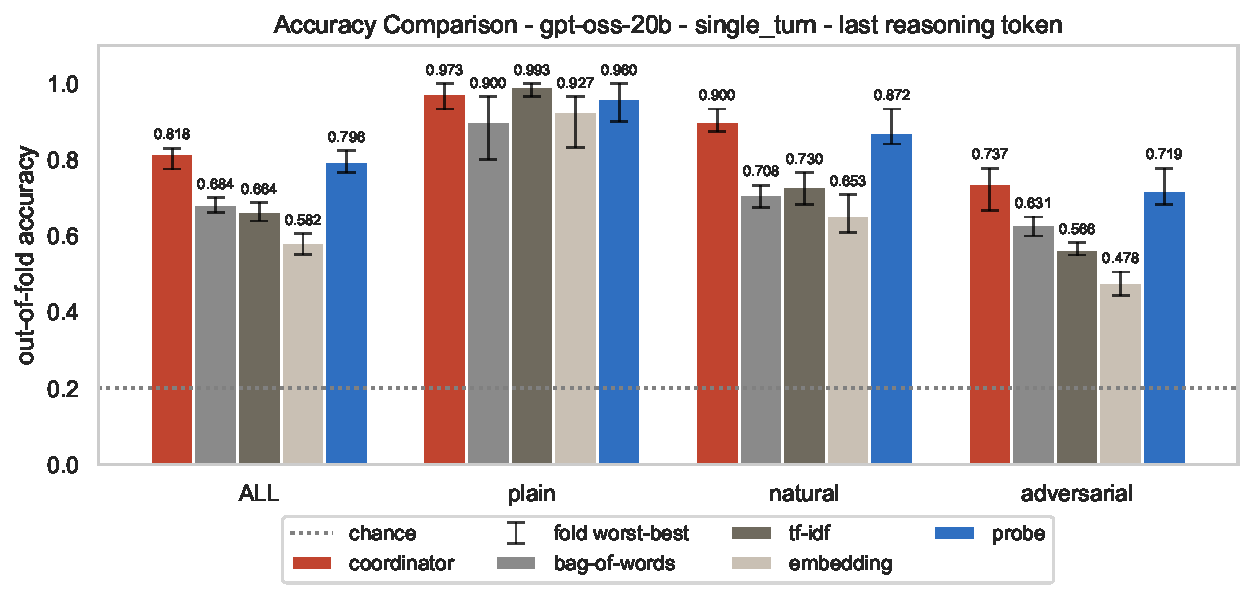
\includegraphics[width=0.85\textwidth]{images/models/gpt-oss-20b_single_turn_reasoning_routers.pdf}
    \caption[Accuracy comparison, gpt-oss-20b, single-turn, probe at the last reasoning token]{Accuracy comparison, gpt-oss-20b, single-turn, probe at the last reasoning token.}
    \label{fig:ch8-gpt-oss-reasoning-routers}
\end{figure}

\subsection{Observations}
\label{subsec:ch8-gpt-oss-observations}

At the last reasoning token, the AUC macro of the probe rises from 0.915 to 0.936. The accuracy of the probe rises from 0.689 to 0.796 on the whole dataset and from 0.601 to 0.719 on the \texttt{adversarial} tier. The probe exceeds all three text-only baselines on the whole dataset and on the \texttt{natural} and \texttt{adversarial} tiers, and its accuracy gets close to the accuracy of the coordinator without exceeding it. The accuracy of the coordinator exceeds the accuracy of the probe by 0.022 on the whole dataset and 0.018 on the \texttt{adversarial} tier. According to the McNemar test, the difference is significant on the whole dataset ($p_{\text{holm}} = 0.026$) but not on the \texttt{adversarial} tier ($p_{\text{holm}} = 0.20$).

A possible reason is that, before the last reasoning token, the model has already generated a reasoning output that discusses the sub-agents and reaches a conclusion. The hidden state during reasoning summarizes the input and the reasoning generated so far, and it is updated as the reasoning proceeds towards a final answer \cite{luStreamingHallucinationDetection2026}. The hidden state at the last reasoning token may therefore be skewed towards the sub-agent the model chose. This does not happen for the other seven models, where the probe reads the hidden state before any output is generated. This reading is consistent with the fraction of samples where the probe predicts the same sub-agent as the coordinator, which rises from 0.672 at the last prompt token to 0.866 at the last reasoning token. A probe trained from this state may therefore mostly learn the decision of the coordinator, including its errors, which would explain why its accuracy approaches the accuracy of the coordinator without exceeding it.

For GPT-OSS 20B, the hidden state at the last prompt token may not yet encode enough information to predict the choice of the sub-agent, because that choice depends on the reasoning generated afterward. The hidden state at the last reasoning token, in contrast, may already reflect that choice, since the reasoning that leads to it has already been generated.

\subsection{Effect on the Rest of the Analysis}
\label{subsec:ch8-gpt-oss-exclusion}

Both probe positions examined in this section have a limitation for GPT-OSS 20B. At the last prompt token, the hidden state may not yet encode the choice of the sub-agent, because that choice may be formed during the reasoning output. At the last reasoning token, the hidden state may already reflect that choice, so the probe may mostly learn the decision of the coordinator, including its errors.

The results of GPT-OSS 20B are therefore excluded from Sections~\ref{sec:ch8-overview} to~\ref{sec:ch8-error-flag}, so that they are not pooled with the results of the other seven models.

\FloatBarrier
